\documentclass[12pt]{article}


\begin{document}
Notre projet dispose de plusieurs formes : 
\begin{itemize}
\item {Sphère}
\item {Plan}
\item {Triangle}
\item {Icosphere}
\item {...}
\end{itemize}
Les formes faites avec des triangles héritent de la classe ShapeTriangleUtil qui factorise les méthodes communes. Les formes définies avec des relations mathématiques héritent de ShapeUtil. Toutes les formes implémentent l'interface Shape qui est l'interface définissant une forme. 

\begin{figure}[ht]
\begin{center}
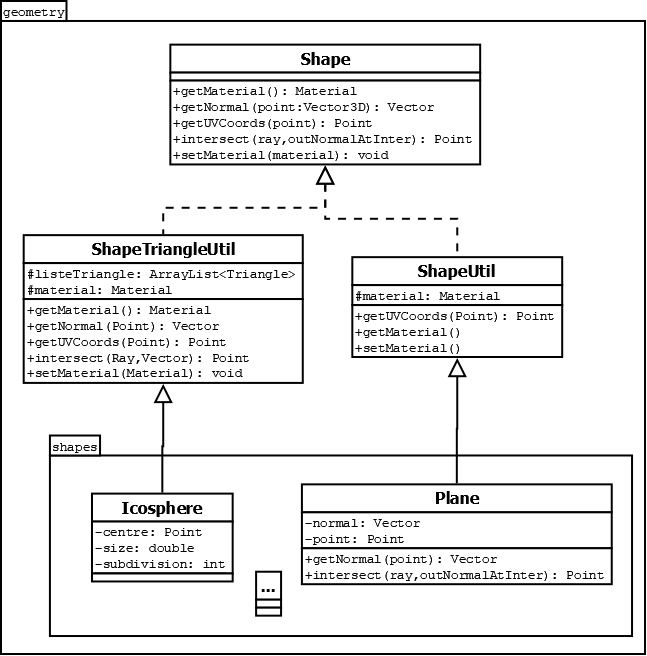
\includegraphics[width = 0.8 \textwidth]{diagrammes/package_geometry.png}
\caption{Diagramme du package geometry}
\end{center}
\end{figure}
\FloatBarrier
\end{document}